% =============================================================================
% THU THẬP TIN TỨC TỰ ĐỘNG VỚI AI-POWERED CRAWLER
% =============================================================================

\section{Thu thập Tin tức Tự động với AI-Powered Crawler}

\begin{figure}[H]
\centering
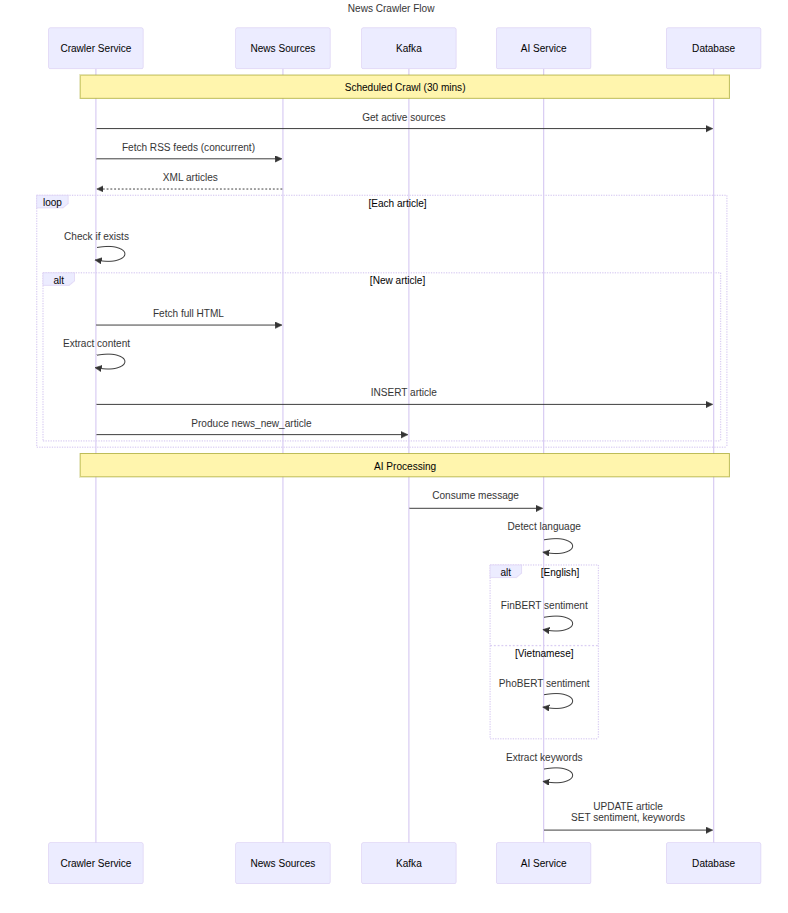
\includegraphics[width=\textwidth]{sequence/sequence_crawler_flow.png}
\caption{Sequence Diagram: News Crawler Flow với Kafka Event-Driven}
\label{fig:seq-crawler}
\end{figure}

\subsection{Bối cảnh}

Bạn cần thu thập tin tức tài chính từ hàng trăm website khác nhau. Một số trang sử dụng JavaScript để hiển thị nội dung (Single Page App), một số thường xuyên thay đổi cấu trúc HTML. Các công cụ crawler truyền thống như XPath hoặc CSS Selector liên tục bị lỗi, cần cập nhật lại thủ công, gây tốn kém chi phí bảo trì.

Yêu cầu hệ thống có thể:
\begin{itemize}
    \item Tự thích ứng với thay đổi cấu trúc trang
    \item Phân tích nội dung chính của bài viết (tiêu đề, ngày, nội dung) từ HTML hỗn tạp
    \item Vận hành ổn định khi scale lên hàng nghìn trang cần thu thập
\end{itemize}

\subsection{Vấn đề với Crawler Truyền thống}

\noindent\textbf{Lý do crawler truyền thống dễ bị lỗi:}

\begin{enumerate}
    \item \textbf{Phụ thuộc vào cấu trúc HTML}:
    \begin{itemize}
        \item XPath và CSS Selector cố định sẽ lỗi khi website thay đổi layout
        \item Một class name thay đổi có thể làm hỏng toàn bộ crawler
        \item Không có khả năng tự phục hồi
    \end{itemize}
    
    \item \textbf{JavaScript Rendering}:
    \begin{itemize}
        \item Single Page Applications (SPA) render content bằng JavaScript
        \item Traditional crawlers chỉ lấy được HTML tĩnh ban đầu
        \item Cần headless browser tốn tài nguyên
    \end{itemize}
    
    \item \textbf{Chi phí bảo trì cao}:
    \begin{itemize}
        \item Mỗi website cần cấu hình selector riêng
        \item Phải monitor và update thủ công khi website thay đổi
        \item Không scale được với hàng trăm nguồn tin
    \end{itemize}
\end{enumerate}

\subsection{Giải pháp trong mã nguồn: Crawler Service (Golang)}

\noindent\textbf{Kiến trúc Crawler Service:}

Crawler Service được viết bằng Golang với các đặc điểm sau:
\begin{itemize}
    \item \textbf{Multi-source crawling}: Thu thập tin tức từ RSS feeds của nhiều nguồn khác nhau (CoinDesk, CoinTelegraph, VNExpress, VnEconomy)
    
    \item \textbf{Event-driven architecture}: Sử dụng Kafka để gửi bài viết mới đến AI Service để phân tích sentiment và extract keywords
    
    \item \textbf{AI-powered selector learning}: Tích hợp Gemini AI để tự động phân tích và học CSS selectors cho mỗi nguồn tin mới, giảm thiểu công việc cấu hình thủ công
    
    \item \textbf{Concurrent processing}: Sử dụng goroutines của Golang để crawl nhiều sources đồng thời, tối ưu throughput
    
    \item \textbf{Error handling}: Retry với exponential backoff khi có lỗi network hoặc parsing
\end{itemize}

Kiến trúc code (file: \texttt{crawler-service/internal/crawler/crawler.go}) sử dụng struct \texttt{Service} với dependencies injection (config, database, Kafka producer). Method \texttt{CrawlOnce()} thực hiện một chu kỳ crawl cho tất cả sources, sử dụng \texttt{sync.WaitGroup} và \texttt{atomic.AddInt64} để đếm số bài viết crawled thành công.

\noindent\textbf{Kafka Integration:}

Crawler Service đóng vai trò Producer trong Kafka architecture. Mỗi khi crawl được bài viết mới, service sẽ:
\begin{itemize}
    \item Marshal article data (ID, title, content, timestamp) thành JSON
    \item Produce message vào Kafka topic \texttt{news\_new\_article}
    \item AI Service (Consumer) sẽ nhận và xử lý message này
\end{itemize}

Implementation sử dụng Confluent Kafka library cho Golang với cấu hình: topic partitioning tự động (\texttt{PartitionAny}), async produce để không block crawler thread.

\noindent\textbf{Gemini AI cho CSS Selector Analysis:}

Gemini AI Client (file: \texttt{ai-service-python/internal/gemini/gemini\_client.py}) sử dụng Google Generative AI SDK với model \texttt{gemini-1.5-flash}. Workflow khi thêm nguồn tin mới:

\begin{enumerate}
    \item Crawler gửi HTML sample đến AI Service qua Kafka topic \texttt{news\_analyze\_css\_selector}
    \item Gemini AI phân tích cấu trúc HTML và đề xuất CSS selectors phù hợp cho: title, content, author, date
    \item Selectors được validate và lưu vào database (bảng \texttt{sources})
    \item Các lần crawl sau sẽ sử dụng selectors đã học này
    \item Nếu selector fail (accuracy < 70\%), tự động trigger re-analysis
\end{enumerate}

\subsection{AI-based Sentiment Analysis}

\noindent\textbf{AI Service với FinBERT và PhoBERT:}

AI Service sử dụng các pre-trained transformer models cho sentiment analysis đa ngôn ngữ:

\begin{itemize}
    \item \textbf{FinBERT} (model: \texttt{yiyanghkust/finbert-tone}):
    \begin{itemize}
        \item Chuyên biệt cho văn bản tài chính tiếng Anh
        \item 3 labels: positive, neutral, negative
        \item Max length: 512 tokens
        \item Output: sentiment score + attention weights
    \end{itemize}
    
    \item \textbf{PhoBERT} (model: \texttt{wonrax/phobert-base-vietnamese-sentiment}):
    \begin{itemize}
        \item Tối ưu cho tiếng Việt
        \item Sử dụng underthesea cho word tokenization
        \item Max length: 256 tokens
        \item Support dấu thanh và ký tự đặc biệt tiếng Việt
    \end{itemize}
    
    \item \textbf{Pipeline}:
    \begin{itemize}
        \item Detect language với langdetect library
        \item Chọn model phù hợp (en → FinBERT, vi → PhoBERT)
        \item Tokenize và inference
        \item Extract attention weights cho keyword extraction
    \end{itemize}
\end{itemize}

\noindent\textbf{Attention-based Keyword Extraction:}

Hệ thống sử dụng attention mechanism của BERT models để extract keywords quan trọng:

\begin{itemize}
    \item Lấy attention weights từ last layer của model
    \item Average attention qua tất cả heads
    \item Tính attention của [CLS] token đối với các tokens khác
    \item Filter stopwords và tokens ngắn (< 3 ký tự)
    \item Sort theo attention weight và lấy top-K keywords
\end{itemize}

Ví dụ: Bài báo về "Bitcoin ETF approval by SEC" sẽ extract keywords: \textit{bitcoin, etf, approval, sec, regulation} dựa trên attention scores cao nhất.

\noindent\textbf{Kafka Consumer cho AI Processing:}

AI Service đóng vai trò Consumer, lắng nghe Kafka topics để xử lý:
\begin{itemize}
    \item \texttt{news\_new\_article}: Phân tích sentiment cho bài viết mới
    \item \texttt{news\_analyze\_css\_selector}: Gemini AI phân tích HTML structure
    \item Batch processing: Process nhiều messages cùng lúc để tối ưu GPU utilization
    \item Error handling: Failed messages được retry hoặc move vào dead-letter queue
\end{itemize}

\textbf{Lưu ý:} Chi tiết về AI Prediction Pipeline với XGBoost và SHAP Explainable AI được trình bày trong Chapter 4.

\subsection{So sánh Rule-based vs AI-based Parser}

\begin{table}[H]
\centering
\caption{So sánh các phương pháp trích xuất nội dung}
\begin{tabular}{|p{3cm}|p{5cm}|p{5cm}|}
\hline
\textbf{Tiêu chí} & \textbf{Rule-based (XPath/CSS)} & \textbf{AI-based (LLM/ML)} \\
\hline
Độ chính xác ban đầu & Cao (nếu selector đúng) & Trung bình-Cao \\
\hline
Khả năng thích ứng & Thấp - phải update thủ công & Cao - tự học cấu trúc mới \\
\hline
Chi phí vận hành & Cao (bảo trì liên tục) & Thấp (sau khi train) \\
\hline
Tốc độ & Rất nhanh & Chậm hơn (inference time) \\
\hline
Resource & Thấp & Cao (GPU/CPU) \\
\hline
Scale & Khó - mỗi site cần config & Dễ - một model cho nhiều site \\
\hline
\end{tabular}
\end{table}

\subsection{Kiến trúc Crawler đề xuất}

\begin{figure}[H]
\centering
\begin{tikzpicture}[
    node distance=1.2cm,
    box/.style={rectangle, draw, minimum width=2.8cm, minimum height=0.8cm, align=center, font=\small}
]

% Components
\node[box, fill=purple!30] (scheduler) {Crawl Scheduler\\(Cron/Schedule)};
\node[box, fill=orange!30, right=2cm of scheduler] (queue) {URL Queue\\(Redis/RabbitMQ)};
\node[box, fill=blue!30, below=1.5cm of queue] (engine) {Crawler Engine\\(Python/Scrapy)};
\node[box, fill=red!30, left=2cm of engine] (parser) {AI Parser\\(LLM/VADER)};
\node[box, fill=gray!30, below=1.5cm of engine] (store) {Data Store\\(PostgreSQL)};

% Arrows
\draw[->] (scheduler) -- node[above]{\tiny URLs} (queue);
\draw[->] (queue) -- node[right]{\tiny Fetch} (engine);
\draw[->] (engine) -- node[above]{\tiny HTML} (parser);
\draw[->] (parser) -- node[left]{\tiny Parsed Data} (store);
\draw[->] (engine) -- node[right]{\tiny Raw Data} (store);

\end{tikzpicture}
\caption{Kiến trúc Crawler với AI Parser}
\end{figure}

\subsection{Kết luận}

\textbf{Khi nào dùng AI-based parser?}
\begin{itemize}
    \item Thu thập từ nhiều nguồn (>50 websites)
    \item Website thường xuyên thay đổi cấu trúc
    \item Cần extract semantic meaning, không chỉ text
    \item Budget cho AI inference không phải vấn đề
\end{itemize}

\textbf{Khi nào dùng Rule-based?}
\begin{itemize}
    \item Số lượng nguồn ít, ổn định (<10)
    \item Website có cấu trúc chuẩn, ít thay đổi
    \item Cần tốc độ cao, real-time crawling
    \item Resource hạn chế
\end{itemize}

